\documentclass[a4paper]{book}
\usepackage{a4wide}
\usepackage{makeidx}
\usepackage{fancyhdr}
\usepackage{graphicx}
\usepackage{multicol}
\usepackage{float}
\usepackage{textcomp}
\usepackage{alltt}
\usepackage{doxygen}
\makeindex
\setcounter{tocdepth}{1}
\renewcommand{\footrulewidth}{0.4pt}
\begin{document}
\begin{titlepage}
\vspace*{7cm}
\begin{center}
{\Large UG\_\-RESCUER Reference Manual\\[1ex]\large 1.0 }\\
\vspace*{1cm}
{\large Generated by Doxygen 1.3.7}\\
\vspace*{0.5cm}
{\small Thu Jul 20 12:10:17 2006}\\
\end{center}
\end{titlepage}
\clearemptydoublepage
\pagenumbering{roman}
\tableofcontents
\clearemptydoublepage
\pagenumbering{arabic}
\chapter{UG\_\-RESCUER Hierarchical Index}
\section{UG\_\-RESCUER Class Hierarchy}
This inheritance list is sorted roughly, but not completely, alphabetically:\begin{CompactList}
\item \contentsline{section}{DGSAcceptor}{\pageref{classDGSAcceptor}}{}
\item \contentsline{section}{DGSTask}{\pageref{classDGSTask}}{}
\begin{CompactList}
\item DGSNetwork\-Handler\item \contentsline{section}{Serial\-Console}{\pageref{classSerialConsole}}{}
\item \contentsline{section}{Serial\-Handler}{\pageref{classSerialHandler}}{}
\end{CompactList}
\item \contentsline{section}{Serial\-Feedback\-Data}{\pageref{classSerialFeedbackData}}{}
\item \contentsline{section}{Takes}{\pageref{classTakes}}{}
\end{CompactList}

\chapter{UG\_\-RESCUER Class Index}
\section{UG\_\-RESCUER Class List}
Here are the classes, structs, unions and interfaces with brief descriptions:\begin{CompactList}
\item\contentsline{section}{{\bf Serial\-Console} (Provides console like access to the serial port ===================================================================================== )}{\pageref{classSerialConsole}}{}
\item\contentsline{section}{{\bf Serial\-Handler} (Implements the Serial Adaptor ---------------------------------------------------------------------------- )}{\pageref{classSerialHandler}}{}
\end{CompactList}

\chapter{UG\_\-RESCUER File Index}
\section{UG\_\-RESCUER File List}
Here is a list of all documented files with brief descriptions:\begin{CompactList}
\item\contentsline{section}{{\bf DGSDriver.cpp} }{\pageref{DGSDriver_8cpp}}{}
\item\contentsline{section}{{\bf DGSDriver.h} }{\pageref{DGSDriver_8h}}{}
\item\contentsline{section}{{\bf DGSTask.h} }{\pageref{DGSTask_8h}}{}
\item\contentsline{section}{{\bf Serial\-Console.cpp} }{\pageref{SerialConsole_8cpp}}{}
\item\contentsline{section}{{\bf Serial\-Console.h} }{\pageref{SerialConsole_8h}}{}
\item\contentsline{section}{{\bf Serial\-Handler.cpp} }{\pageref{SerialHandler_8cpp}}{}
\item\contentsline{section}{{\bf Serial\-Handler.h} }{\pageref{SerialHandler_8h}}{}
\end{CompactList}

\chapter{UG\_\-RESCUER Page Index}
\section{UG\_\-RESCUER Related Pages}
Here is a list of all related documentation pages:\begin{CompactList}
\item \contentsline{section}{Todo List}{\pageref{todo}}{}

\end{CompactList}

\chapter{UG\_\-RESCUER Class Documentation}
\section{DGSTask Class Reference}
\label{classDGSTask}\index{DGSTask@{DGSTask}}
{\tt \#include $<$DGSTask.h$>$}

Inheritance diagram for DGSTask::\begin{figure}[H]
\begin{center}
\leavevmode
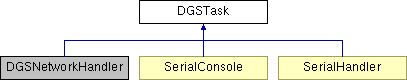
\includegraphics[height=2cm]{classDGSTask}
\end{center}
\end{figure}
\subsection*{Public Member Functions}
\begin{CompactItemize}
\item 
{\bf DGSTask} ()
\item 
virtual int {\bf Is\-Alive} ()
\end{CompactItemize}


\subsection{Detailed Description}
Extents ACE\_\-Task and implements some usefull commands for the Dexterous Grasping System enviroment 



\subsection{Constructor \& Destructor Documentation}
\index{DGSTask@{DGSTask}!DGSTask@{DGSTask}}
\index{DGSTask@{DGSTask}!DGSTask@{DGSTask}}
\subsubsection{\setlength{\rightskip}{0pt plus 5cm}DGSTask::DGSTask ()\hspace{0.3cm}{\tt  [inline]}}\label{classDGSTask_a0}


DGSTask Constructor 

\subsection{Member Function Documentation}
\index{DGSTask@{DGSTask}!IsAlive@{IsAlive}}
\index{IsAlive@{IsAlive}!DGSTask@{DGSTask}}
\subsubsection{\setlength{\rightskip}{0pt plus 5cm}virtual int DGSTask::Is\-Alive ()\hspace{0.3cm}{\tt  [inline, virtual]}}\label{classDGSTask_a1}


Is\-Alive Prints a Message signaling that is alive. As virtual function can be overwrited by descendant classes to personalize their alive messages \begin{Desc}
\item[Returns:]\end{Desc}


Reimplemented in {\bf Serial\-Console} {\rm (p.\,\pageref{classSerialConsole_a4})}.

The documentation for this class was generated from the following file:\begin{CompactItemize}
\item 
{\bf DGSTask.h}\end{CompactItemize}

\section{Serial\-Console Class Reference}
\label{classSerialConsole}\index{SerialConsole@{SerialConsole}}
{\tt \#include $<$Serial\-Console.h$>$}

Inheritance diagram for Serial\-Console::\begin{figure}[H]
\begin{center}
\leavevmode
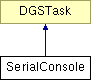
\includegraphics[height=2cm]{classSerialConsole}
\end{center}
\end{figure}
\subsection*{Public Member Functions}
\begin{CompactItemize}
\item 
{\bf Serial\-Console} ()
\item 
{\bf $\sim$Serial\-Console} ()
\item 
virtual int {\bf svc} ()
\item 
int {\bf set\-Commands\-Consumer} ({\bf DGSTask} $\ast$consumer)
\item 
virtual int {\bf Is\-Alive} ()
\end{CompactItemize}


\subsection{Detailed Description}
Provides console like access to the serial port. 



\subsection{Constructor \& Destructor Documentation}
\index{SerialConsole@{Serial\-Console}!SerialConsole@{SerialConsole}}
\index{SerialConsole@{SerialConsole}!SerialConsole@{Serial\-Console}}
\subsubsection{\setlength{\rightskip}{0pt plus 5cm}Serial\-Console::Serial\-Console ()}\label{classSerialConsole_a0}


Serial\-Console constructor \index{SerialConsole@{Serial\-Console}!~SerialConsole@{$\sim$SerialConsole}}
\index{~SerialConsole@{$\sim$SerialConsole}!SerialConsole@{Serial\-Console}}
\subsubsection{\setlength{\rightskip}{0pt plus 5cm}Serial\-Console::$\sim${\bf Serial\-Console} ()}\label{classSerialConsole_a1}


{\bf Serial\-Console::$\sim$Serial\-Console}{\rm (p.\,\pageref{classSerialConsole_a1})} Destructor 

\subsection{Member Function Documentation}
\index{SerialConsole@{Serial\-Console}!IsAlive@{IsAlive}}
\index{IsAlive@{IsAlive}!SerialConsole@{Serial\-Console}}
\subsubsection{\setlength{\rightskip}{0pt plus 5cm}virtual int Serial\-Console::Is\-Alive ()\hspace{0.3cm}{\tt  [inline, virtual]}}\label{classSerialConsole_a4}


Is\-Alive Prints a messages signaling that is alive

\begin{Desc}
\item[Returns:]\end{Desc}


Reimplemented from {\bf DGSTask} {\rm (p.\,\pageref{classDGSTask_a1})}.\index{SerialConsole@{Serial\-Console}!setCommandsConsumer@{setCommandsConsumer}}
\index{setCommandsConsumer@{setCommandsConsumer}!SerialConsole@{Serial\-Console}}
\subsubsection{\setlength{\rightskip}{0pt plus 5cm}int Serial\-Console::set\-Commands\-Consumer ({\bf DGSTask} $\ast$ {\em consumer})\hspace{0.3cm}{\tt  [inline]}}\label{classSerialConsole_a3}


set\-Commands\-Consumer Set the pointer to the Serial handler accepting console messages

\begin{Desc}
\item[Parameters:]
\begin{description}
\item[{\em consumer}]The pointer to the hander implementing a message queue that can be used to input messages using the \char`\"{}put\char`\"{} function\end{description}
\end{Desc}
\begin{Desc}
\item[Returns:]\end{Desc}
\index{SerialConsole@{Serial\-Console}!svc@{svc}}
\index{svc@{svc}!SerialConsole@{Serial\-Console}}
\subsubsection{\setlength{\rightskip}{0pt plus 5cm}int Serial\-Console::svc ()\hspace{0.3cm}{\tt  [virtual]}}\label{classSerialConsole_a2}


svc Internal console loop. Read keyboar commands

\begin{Desc}
\item[Returns:]\end{Desc}


The documentation for this class was generated from the following files:\begin{CompactItemize}
\item 
{\bf Serial\-Console.h}\item 
{\bf Serial\-Console.cpp}\end{CompactItemize}

\section{Serial\-Handler Class Reference}
\label{classSerialHandler}\index{SerialHandler@{SerialHandler}}
Implements the Serial Adaptor ----------------------------------------------------------------------------.  


{\tt \#include $<$Serial\-Handler.h$>$}

\subsection*{Public Member Functions}
\begin{CompactItemize}
\item 
{\bf Serial\-Handler} (void)
\begin{CompactList}\small\item\em {\bf Serial\-Handler::Serial\-Handler}{\rm (p.\,\pageref{classSerialHandler_a0})} ----------------------------------------------------------------------------. \item\end{CompactList}\item 
{\bf $\sim$Serial\-Handler} (void)
\begin{CompactList}\small\item\em {\bf Serial\-Handler::$\sim$Serial\-Handler}{\rm (p.\,\pageref{classSerialHandler_a1})} Destructor. \item\end{CompactList}\item 
int {\bf initialize} (void)
\begin{CompactList}\small\item\em initialize starts the inizialization of the serial device and attach it to the reading streams. \item\end{CompactList}\item 
virtual int {\bf svc} ()
\begin{CompactList}\small\item\em svc This is the internal loop of the ACETask, it read from the standart input. \item\end{CompactList}\end{CompactItemize}
\subsection*{Protected Member Functions}
\begin{CompactItemize}
\item 
virtual void {\bf handle\_\-read\_\-stream} (const ACE\_\-Asynch\_\-Read\_\-Stream::Result \&result)
\begin{CompactList}\small\item\em handle\_\-read\_\-stream \item\end{CompactList}\item 
virtual void {\bf handle\_\-write\_\-stream} (const ACE\_\-Asynch\_\-Write\_\-Stream::Result \&result)
\begin{CompactList}\small\item\em handle\_\-write\_\-stream \item\end{CompactList}\end{CompactItemize}


\subsection{Detailed Description}
Implements the Serial Adaptor ----------------------------------------------------------------------------. 

-------------------------------------------------------------------------- 



\subsection{Constructor \& Destructor Documentation}
\index{SerialHandler@{Serial\-Handler}!SerialHandler@{SerialHandler}}
\index{SerialHandler@{SerialHandler}!SerialHandler@{Serial\-Handler}}
\subsubsection{\setlength{\rightskip}{0pt plus 5cm}Serial\-Handler::Serial\-Handler (void)}\label{classSerialHandler_a0}


{\bf Serial\-Handler::Serial\-Handler}{\rm (p.\,\pageref{classSerialHandler_a0})} ----------------------------------------------------------------------------. 

-------------------------------------------------------------------------- \index{SerialHandler@{Serial\-Handler}!~SerialHandler@{$\sim$SerialHandler}}
\index{~SerialHandler@{$\sim$SerialHandler}!SerialHandler@{Serial\-Handler}}
\subsubsection{\setlength{\rightskip}{0pt plus 5cm}Serial\-Handler::$\sim${\bf Serial\-Handler} (void)}\label{classSerialHandler_a1}


{\bf Serial\-Handler::$\sim$Serial\-Handler}{\rm (p.\,\pageref{classSerialHandler_a1})} Destructor. 

-------------------------------------------------------------------------- 

\begin{Desc}
\item[{\bf Todo}]close correctly all the streams ----------------------------------------------------------------------------\end{Desc}


\subsection{Member Function Documentation}
\index{SerialHandler@{Serial\-Handler}!handle_read_stream@{handle\_\-read\_\-stream}}
\index{handle_read_stream@{handle\_\-read\_\-stream}!SerialHandler@{Serial\-Handler}}
\subsubsection{\setlength{\rightskip}{0pt plus 5cm}void Serial\-Handler::handle\_\-read\_\-stream (const ACE\_\-Asynch\_\-Read\_\-Stream::Result \& {\em result})\hspace{0.3cm}{\tt  [protected, virtual]}}\label{classSerialHandler_b0}


handle\_\-read\_\-stream 

-------------------------------------------------------------------------- 

\begin{Desc}
\item[Parameters:]
\begin{description}
\item[{\em result}]---------------------------------------------------------------------------- \end{description}
\end{Desc}
\index{SerialHandler@{Serial\-Handler}!handle_write_stream@{handle\_\-write\_\-stream}}
\index{handle_write_stream@{handle\_\-write\_\-stream}!SerialHandler@{Serial\-Handler}}
\subsubsection{\setlength{\rightskip}{0pt plus 5cm}void Serial\-Handler::handle\_\-write\_\-stream (const ACE\_\-Asynch\_\-Write\_\-Stream::Result \& {\em result})\hspace{0.3cm}{\tt  [protected, virtual]}}\label{classSerialHandler_b1}


handle\_\-write\_\-stream 

-------------------------------------------------------------------------- 

\begin{Desc}
\item[Parameters:]
\begin{description}
\item[{\em result}]---------------------------------------------------------------------------- \end{description}
\end{Desc}
\index{SerialHandler@{Serial\-Handler}!initialize@{initialize}}
\index{initialize@{initialize}!SerialHandler@{Serial\-Handler}}
\subsubsection{\setlength{\rightskip}{0pt plus 5cm}int Serial\-Handler::initialize (void)}\label{classSerialHandler_a2}


initialize starts the inizialization of the serial device and attach it to the reading streams. 

-------------------------------------------------------------------------- 

\begin{Desc}
\item[Returns:]---------------------------------------------------------------------------- \end{Desc}
\index{SerialHandler@{Serial\-Handler}!svc@{svc}}
\index{svc@{svc}!SerialHandler@{Serial\-Handler}}
\subsubsection{\setlength{\rightskip}{0pt plus 5cm}int Serial\-Handler::svc ()\hspace{0.3cm}{\tt  [virtual]}}\label{classSerialHandler_a3}


svc This is the internal loop of the ACETask, it read from the standart input. 

-------------------------------------------------------------------------- 

\begin{Desc}
\item[Returns:]---------------------------------------------------------------------------- \end{Desc}


The documentation for this class was generated from the following files:\begin{CompactItemize}
\item 
{\bf Serial\-Handler.h}\item 
{\bf Serial\-Handler.cpp}\end{CompactItemize}

\chapter{UG\_\-RESCUER File Documentation}
\input{DGSAcceptor_8cpp}
\include{DGSAcceptor_8h}
\section{DGSDriver.cpp File Reference}
\label{DGSDriver_8cpp}\index{DGSDriver.cpp@{DGSDriver.cpp}}
Contains the driver for the Dexterous Grasping System (Three finger gripper).  


{\tt \#include \char`\"{}Serial\-Handler.h\char`\"{}}\par
{\tt \#include \char`\"{}Serial\-Console.h\char`\"{}}\par
{\tt \#include \char`\"{}DGSDriver.h\char`\"{}}\par
\subsection*{Defines}
\begin{CompactItemize}
\item 
\#define {\bf ACE\_\-NTRACE}\ 0\label{DGSDriver_8cpp_a0}

\end{CompactItemize}


\subsection{Detailed Description}
Contains the driver for the Dexterous Grasping System (Three finger gripper). 

=================================================================================

RESCUER - IST-2003-511492 (c) 2004-2008

Improvement of the Emergency Risk Management through Secure Mobile Mechatronic Support to Bomb Disposal and Rescue Operations

\begin{Desc}
\item[Version:]1.0 \end{Desc}
\begin{Desc}
\item[Date:]20-Jun-06 1:10:28 PM ora solare Europa occidentale \end{Desc}
\begin{Desc}
\item[Author:]Carlos Beltran Gonzalez (Carlos), {\tt cbeltran@dist.unige.it} 

Lira-Lab. Revisions:. ===================================================================================\end{Desc}

\section{DGSDriver.h File Reference}
\label{DGSDriver_8h}\index{DGSDriver.h@{DGSDriver.h}}


\subsection{Detailed Description}
RESCUER - IST-2003-511492 (c) 2004-2008

Improvement of the Emergency Risk Management through Secure Mobile Mechatronic Support to Bomb Disposal and Rescue Operations

\begin{Desc}
\item[Version:]1.0 \end{Desc}
\begin{Desc}
\item[Date:]21-Jun-06 1:14:25 PM ora solare Europa occidentale \end{Desc}
\begin{Desc}
\item[Author:]Carlos Beltran Gonzalez (Carlos), {\tt cbeltran@dist.unige.it} 

Lira-Lab Revisions:\end{Desc}

\include{DGSNetworkHandler_8cpp}
\include{DGSNetworkHandler_8h}
\section{DGSTask.h File Reference}
\label{DGSTask_8h}\index{DGSTask.h@{DGSTask.h}}
{\tt \#include $<$ace/Task.h$>$}\par
\subsection*{Classes}
\begin{CompactItemize}
\item 
class {\bf DGSTask}
\end{CompactItemize}


\subsection{Detailed Description}
RESCUER - IST-2003-511492 (c) 2004-2008

Improvement of the Emergency Risk Management through Secure Mobile Mechatronic Support to Bomb Disposal and Rescue Operations

Extents ACE\_\-Task template \begin{Desc}
\item[Version:]1.0 \end{Desc}
\begin{Desc}
\item[Date:]13-Jul-06 12:09:23 PM ora solare Europa occidentale \end{Desc}
\begin{Desc}
\item[Author:]Carlos Beltran Gonzalez (Carlos), {\tt cbeltran@dist.unige.it} 

Lira-Lab Revisions:\end{Desc}

\section{Serial\-Console.cpp File Reference}
\label{SerialConsole_8cpp}\index{SerialConsole.cpp@{SerialConsole.cpp}}
{\tt \#include \char`\"{}Serial\-Console.h\char`\"{}}\par


\subsection{Detailed Description}
RESCUER - IST-2003-511492 (c) 2004-2008

Improvement of the Emergency Risk Management through Secure Mobile Mechatronic Support to Bomb Disposal and Rescue Operations

Provides a text like console to access directly the Serial Handler. It runs its own svc loop reading from the keyboard and puts the command into the {\bf Serial\-Handler}{\rm (p.\,\pageref{classSerialHandler})} ACE\_\-Message\_\-Queue \begin{Desc}
\item[Version:]1.0 \end{Desc}
\begin{Desc}
\item[Date:]26-Jun-06 4:03:17 PM ora solare Europa occidentale \end{Desc}
\begin{Desc}
\item[Author:]Carlos Beltran Gonzalez (Carlos), {\tt cbeltran@dist.unige.it} 

Lira-Lab Revisions:\end{Desc}

\section{Serial\-Console.h File Reference}
\label{SerialConsole_8h}\index{SerialConsole.h@{SerialConsole.h}}
{\tt \#include $<$stdio.h$>$}\par
{\tt \#include $<$string$>$}\par
{\tt \#include \char`\"{}DGSTask.h\char`\"{}}\par
{\tt \#include \char`\"{}DGSDriver.h\char`\"{}}\par
{\tt \#include \char`\"{}Serial\-Feedback\-Data.h\char`\"{}}\par
\subsection*{Classes}
\begin{CompactItemize}
\item 
class {\bf Serial\-Console}
\end{CompactItemize}


\subsection{Detailed Description}
RESCUER - IST-2003-511492 (c) 2004-2008

Improvement of the Emergency Risk Management through Secure Mobile Mechatronic Support to Bomb Disposal and Rescue Operations

Provides a text like console to access directly the Serial Handler. It runs its own svc loop reading from the keyboard and puts the command into the {\bf Serial\-Handler}{\rm (p.\,\pageref{classSerialHandler})} ACE\_\-Message\_\-Queue. \begin{Desc}
\item[Version:]1.0 \end{Desc}
\begin{Desc}
\item[Date:]26-Jun-06 4:06:17 PM ora solare Europa occidentale \end{Desc}
\begin{Desc}
\item[Author:]Carlos Beltran Gonzalez (Carlos), {\tt cbeltran@dist.unige.it} 

Lira-Lab Revisions:\end{Desc}

\section{Serial\-Handler.cpp File Reference}
\label{SerialHandler_8cpp}\index{SerialHandler.cpp@{SerialHandler.cpp}}
{\tt \#include $<$string.h$>$}\par
{\tt \#include \char`\"{}Serial\-Handler.h\char`\"{}}\par


\subsection{Detailed Description}
RESCUER - IST-2003-511492 (c) 2004-2008

Improvement of the Emergency Risk Management through Secure Mobile Mechatronic Support to Bomb Disposal and Rescue Operations

Contains the implementation of the Serial Handler \begin{Desc}
\item[Version:]1.0 \end{Desc}
\begin{Desc}
\item[Date:]21-Jun-06 1:53:39 PM ora solare Europa occidentale \end{Desc}
\begin{Desc}
\item[Author:]Carlos Beltran Gonzalez (Carlos), {\tt cbeltran@dist.unige.it} 

Lira-Lab Revisions: \end{Desc}
\begin{Desc}
\item[{\bf Todo}]Write a correct method of finalization of the system. \end{Desc}

\section{Serial\-Handler.h File Reference}
\label{SerialHandler_8h}\index{SerialHandler.h@{SerialHandler.h}}
Contains the serial handler using the Proactor framework.  


{\tt \#include $<$stdio.h$>$}\par
{\tt \#include $<$string$>$}\par
{\tt \#include \char`\"{}ace/streams.h\char`\"{}}\par
{\tt \#include \char`\"{}ace/Log\_\-Msg.h\char`\"{}}\par
{\tt \#include \char`\"{}ace/OS.h\char`\"{}}\par
{\tt \#include \char`\"{}ace/Proactor.h\char`\"{}}\par
{\tt \#include \char`\"{}ace/Asynch\_\-IO.h\char`\"{}}\par
{\tt \#include \char`\"{}ace/Asynch\_\-IO\_\-Impl.h\char`\"{}}\par
{\tt \#include \char`\"{}ace/Message\_\-Block.h\char`\"{}}\par
{\tt \#include \char`\"{}ace/OS\_\-main.h\char`\"{}}\par
{\tt \#include \char`\"{}ace/TTY\_\-IO.h\char`\"{}}\par
{\tt \#include \char`\"{}ace/Task.h\char`\"{}}\par
{\tt \#include \char`\"{}ace/CDR\_\-Stream.h\char`\"{}}\par
{\tt \#include \char`\"{}ace/DEV\_\-Connector.h\char`\"{}}\par
{\tt \#include \char`\"{}DGSDriver.h\char`\"{}}\par
\subsection*{Classes}
\begin{CompactItemize}
\item 
class {\bf Serial\-Handler}
\begin{CompactList}\small\item\em Implements the Serial Adaptor ----------------------------------------------------------------------------. \item\end{CompactList}\end{CompactItemize}


\subsection{Detailed Description}
Contains the serial handler using the Proactor framework. 

=================================================================================

RESCUER - IST-2003-511492 (c) 2004-2008

Improvement of the Emergency Risk Management through Secure Mobile Mechatronic Support to Bomb Disposal and Rescue Operations

\begin{Desc}
\item[Version:]1.0 \end{Desc}
\begin{Desc}
\item[Date:]21-Jun-06 1:06:18 PM ora solare Europa occidentale \end{Desc}
\begin{Desc}
\item[Author:]Carlos Beltran Gonzalez (Carlos), {\tt cbeltran@dist.unige.it} 

Lira-Lab Revisions: ===================================================================================\end{Desc}

\chapter{UG\_\-RESCUER Page Documentation}
\section{Todo List}\label{todo}
\label{todo__todo000004}
 \begin{description}
\item[Member {\bf Serial\-Handler::$\sim$Serial\-Handler}{\rm (p.\,\pageref{classSerialHandler_a1})}(void) ]close correctly all the streams \end{description}


\label{todo__todo000001}
 \begin{description}
\item[File {\bf DGSDriver.cpp}{\rm (p.\,\pageref{DGSDriver_8cpp})} ]Fix syncronization problems in message queues 

Fix visualization problems in the doxygen documentation \end{description}


\label{todo__todo000003}
 \begin{description}
\item[File {\bf Serial\-Handler.cpp}{\rm (p.\,\pageref{SerialHandler_8cpp})} ]Write a correct method of finalization of the system. \end{description}

\printindex
\end{document}
